\documentclass[11pt]{article}
\usepackage[textwidth=18.0cm, textheight=23.0cm, top=2.0cm]{geometry}
\usepackage{pst-all}
\usepackage{amssymb}
\usepackage{tikz}
\usepackage{underscore}\begin{document}
\pagestyle{empty}


ClassName: \underline{\textbf{Class_10.2bp-25}}
\par
BinSize: \underline{\textbf{100 × 100}}
\par
ReduceSize: \underline{\textbf{100 × 100}}
\par
TypeNum: \underline{\textbf{60}}
\par
Num: \underline{\textbf{60}}
\par
OutS: \underline{\textbf{130000}}
\par
InS: \underline{\textbf{111378}}
\par
Rate: \underline{\textbf{0.857}}
\par
UB: \underline{\textbf{13}}
\par
LB0: \underline{\textbf{13}}
\par
LB: \underline{\textbf{13}}
\par
LBWithCut: \underline{\textbf{13}}
\par
NodeCut: \underline{\textbf{0}}
\par
ExtendedNodeCnt: \underline{\textbf{1}}
\par
GenNodeCnt: \underline{\textbf{1}}
\par
PrimalNode: \underline{\textbf{0}}
\par
ColumnCount: \underline{\textbf{13}}
\par
TotalCutCount: \underline{\textbf{0}}
\par
RootCutCount: \underline{\textbf{0}}
\par
LPSolverCnt: \underline{\textbf{1}}
\par
PricingSolverCnt: \underline{\textbf{0}}
\par
BranchAndBoundNum: \underline{\textbf{1}}
\par
isOpt: \underline{\textbf{true}}
\par
TimeOnInitSolution: \underline{\textbf{600.000 s}}
\par
TimeOnPrimal: \underline{\textbf{0.000 s}}
\par
TimeOnPricing: \underline{\textbf{0.000 s}}
\par
TimeOnRmp: \underline{\textbf{0.062 s}}
\par
TotalTime: \underline{\textbf{600.328 s}}
\par
\newpage


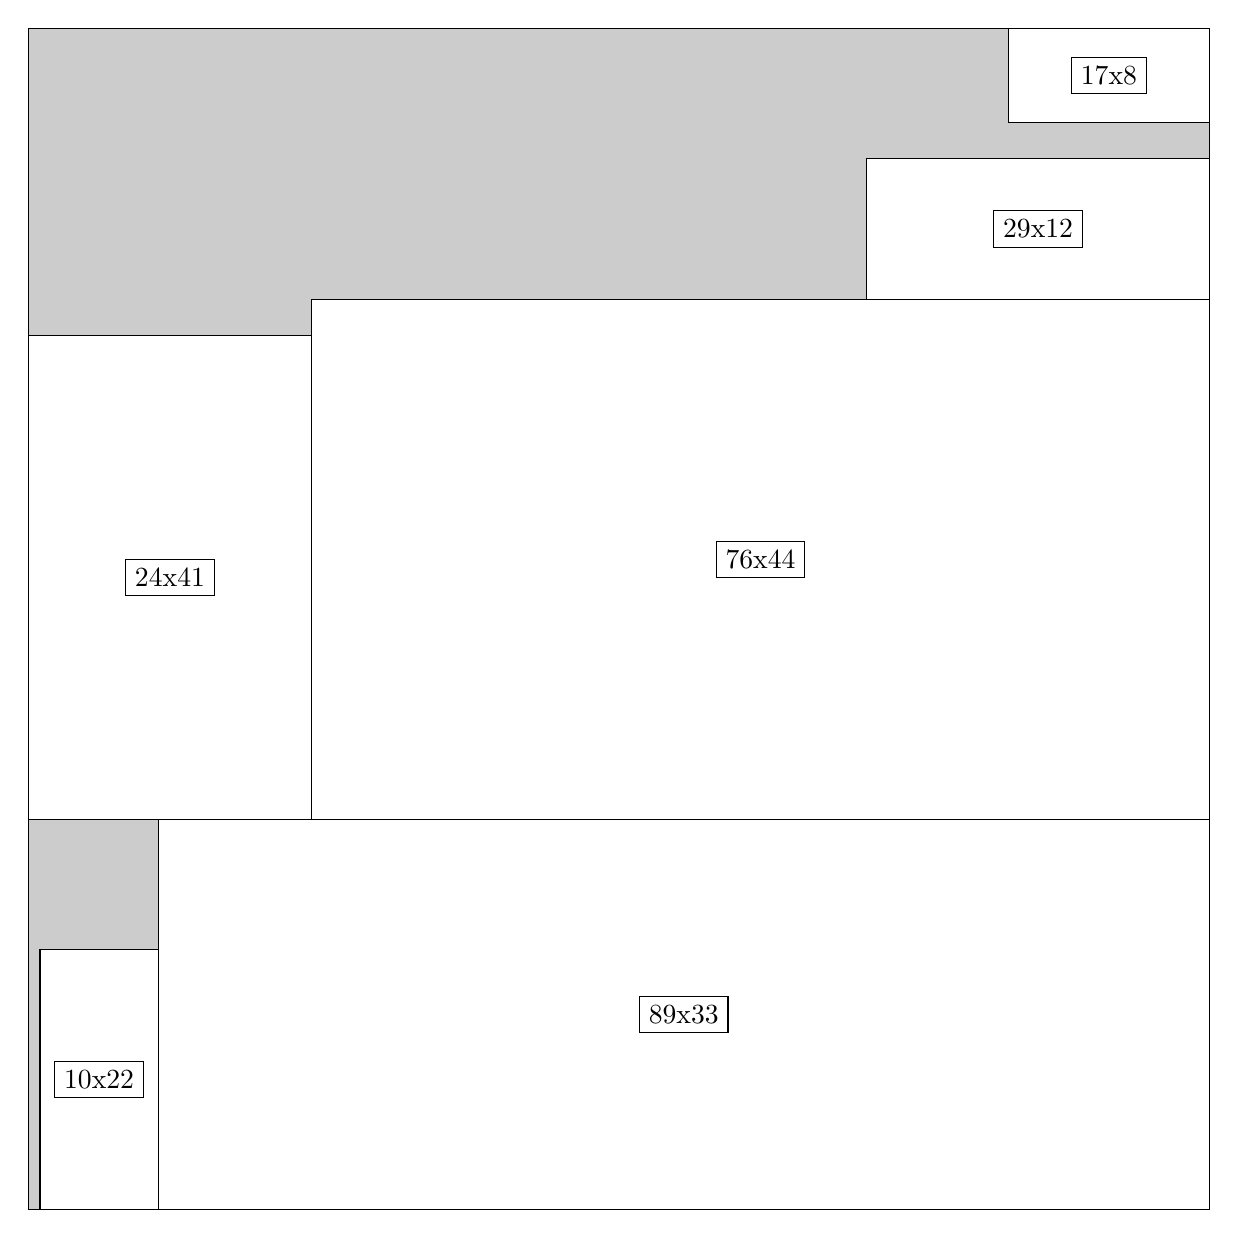
\begin{tikzpicture}[shorten >=1pt,scale=1.0,every node/.style={scale=1.0},->]
\tikzstyle{vertex}=[circle,fill=black!25,minimum size=14pt,inner sep=0pt]
\filldraw[fill=gray!40!white, draw=black] (0,0) rectangle (15.0,15.0);
\foreach \name/\x/\y/\w/\h in {89x33/1.65/0.0/13.35/4.95,10x22/0.15/0.0/1.5/3.3,76x44/3.5999999999999996/4.95/11.4/6.6,29x12/10.65/11.549999999999999/4.35/1.7999999999999998,24x41/0.0/4.95/3.5999999999999996/6.1499999999999995,17x8/12.45/13.799999999999999/2.55/1.2}
\filldraw[fill=white!40!white, draw=black] (\x,\y) rectangle node[draw] (\name) {\name} ++(\w,\h);
\end{tikzpicture}


w =89 , h =33 , x =11 , y =0 , v =2937
\par
w =10 , h =22 , x =1 , y =0 , v =220
\par
w =76 , h =44 , x =24 , y =33 , v =3344
\par
w =29 , h =12 , x =71 , y =77 , v =348
\par
w =24 , h =41 , x =0 , y =33 , v =984
\par
w =17 , h =8 , x =83 , y =92 , v =136
\par
\newpage


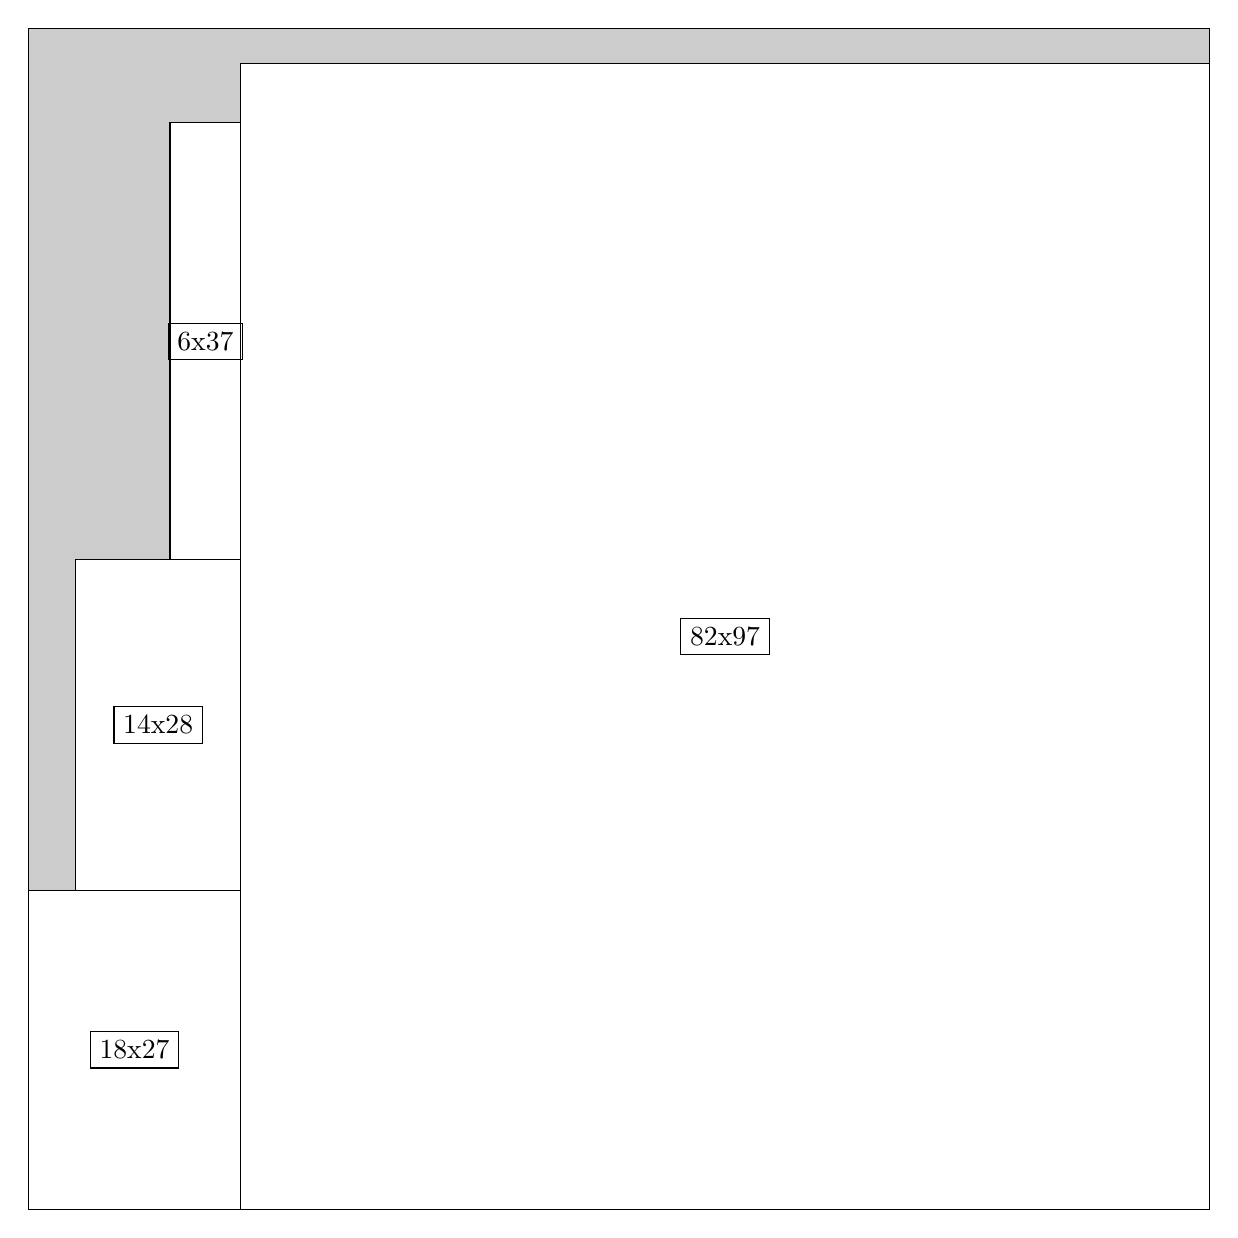
\begin{tikzpicture}[shorten >=1pt,scale=1.0,every node/.style={scale=1.0},->]
\tikzstyle{vertex}=[circle,fill=black!25,minimum size=14pt,inner sep=0pt]
\filldraw[fill=gray!40!white, draw=black] (0,0) rectangle (15.0,15.0);
\foreach \name/\x/\y/\w/\h in {82x97/2.6999999999999997/0.0/12.299999999999999/14.549999999999999,18x27/0.0/0.0/2.6999999999999997/4.05,14x28/0.6/4.05/2.1/4.2,6x37/1.7999999999999998/8.25/0.8999999999999999/5.55}
\filldraw[fill=white!40!white, draw=black] (\x,\y) rectangle node[draw] (\name) {\name} ++(\w,\h);
\end{tikzpicture}


w =82 , h =97 , x =18 , y =0 , v =7954
\par
w =18 , h =27 , x =0 , y =0 , v =486
\par
w =14 , h =28 , x =4 , y =27 , v =392
\par
w =6 , h =37 , x =12 , y =55 , v =222
\par
\newpage


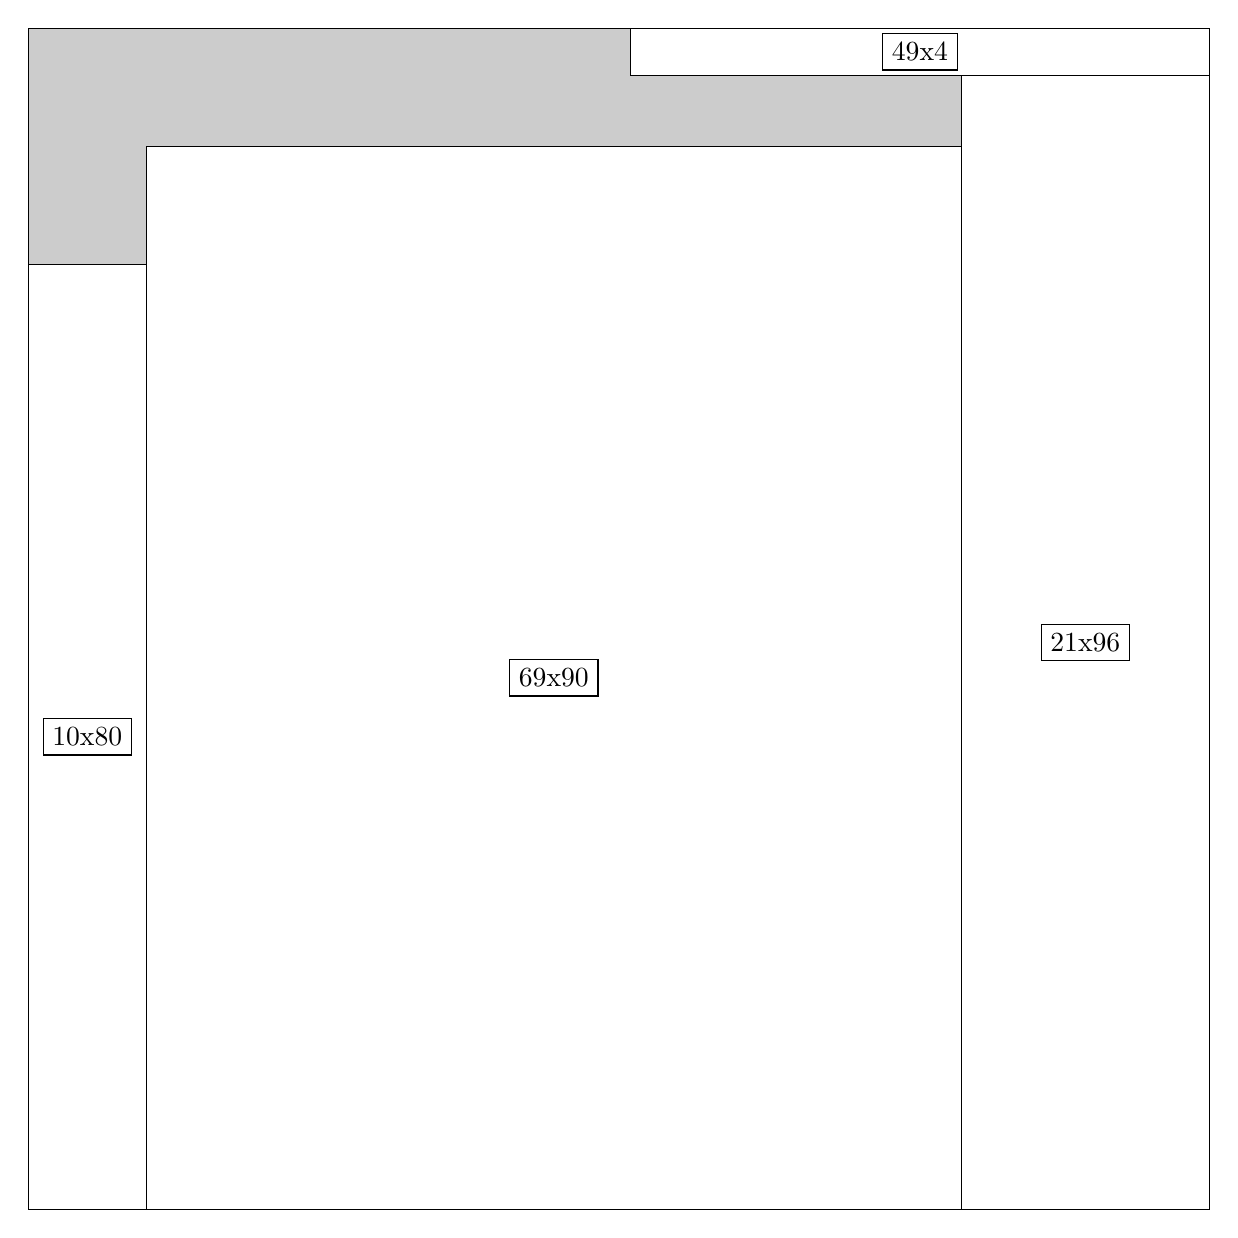
\begin{tikzpicture}[shorten >=1pt,scale=1.0,every node/.style={scale=1.0},->]
\tikzstyle{vertex}=[circle,fill=black!25,minimum size=14pt,inner sep=0pt]
\filldraw[fill=gray!40!white, draw=black] (0,0) rectangle (15.0,15.0);
\foreach \name/\x/\y/\w/\h in {21x96/11.85/0.0/3.15/14.399999999999999,69x90/1.5/0.0/10.35/13.5,10x80/0.0/0.0/1.5/12.0,49x4/7.6499999999999995/14.399999999999999/7.35/0.6}
\filldraw[fill=white!40!white, draw=black] (\x,\y) rectangle node[draw] (\name) {\name} ++(\w,\h);
\end{tikzpicture}


w =21 , h =96 , x =79 , y =0 , v =2016
\par
w =69 , h =90 , x =10 , y =0 , v =6210
\par
w =10 , h =80 , x =0 , y =0 , v =800
\par
w =49 , h =4 , x =51 , y =96 , v =196
\par
\newpage


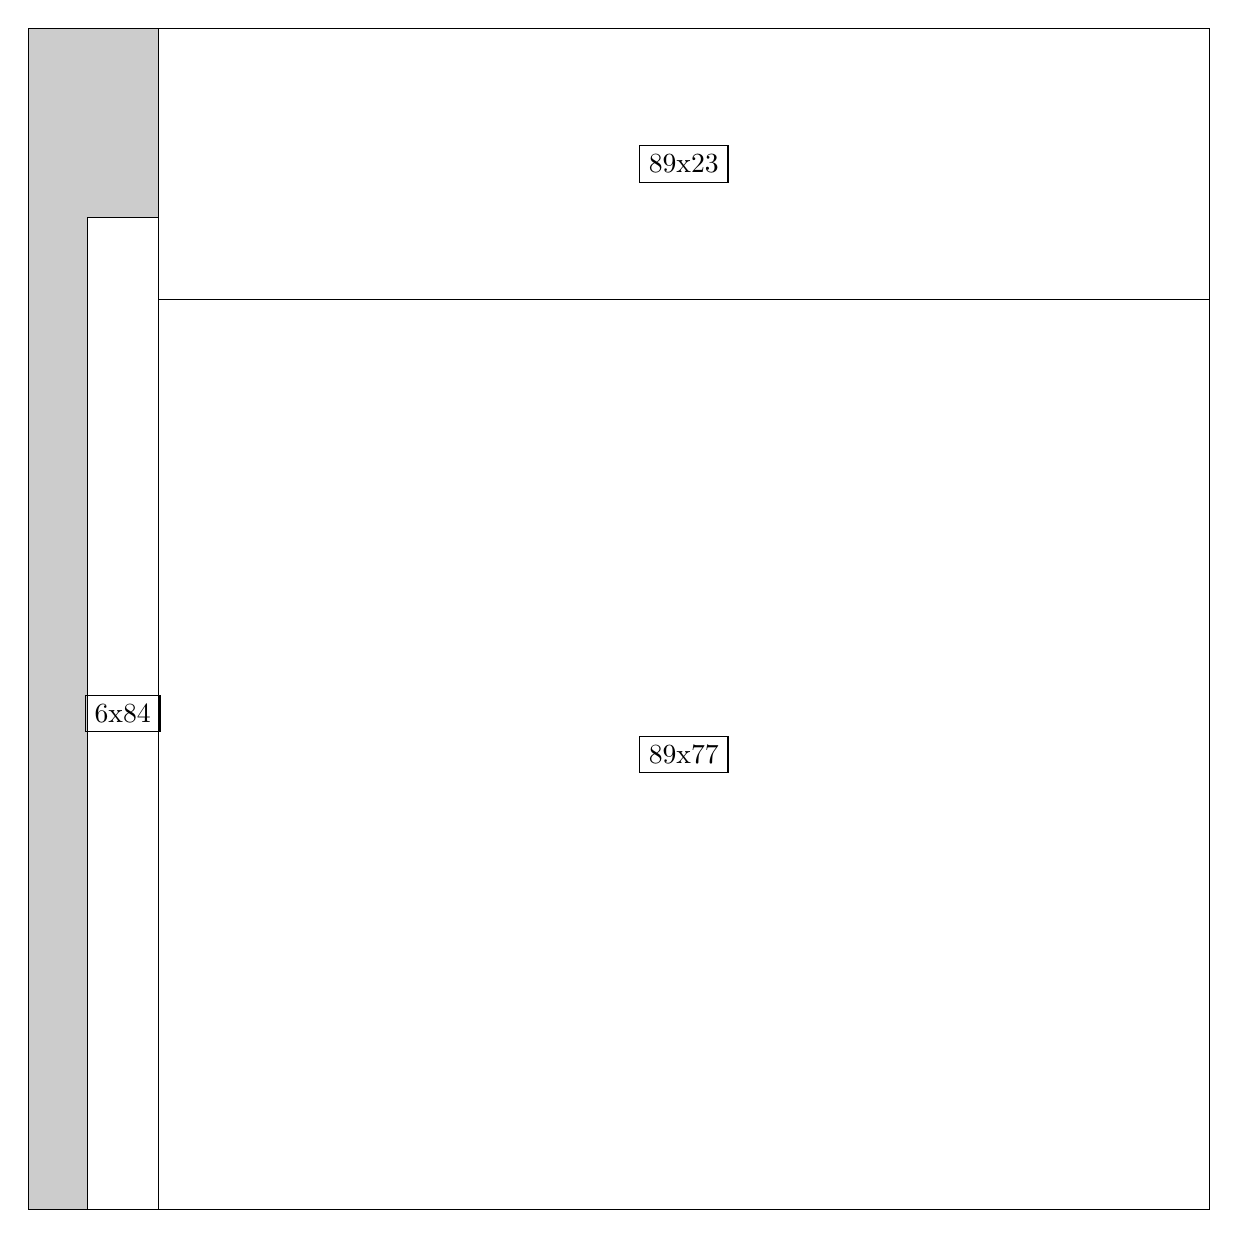
\begin{tikzpicture}[shorten >=1pt,scale=1.0,every node/.style={scale=1.0},->]
\tikzstyle{vertex}=[circle,fill=black!25,minimum size=14pt,inner sep=0pt]
\filldraw[fill=gray!40!white, draw=black] (0,0) rectangle (15.0,15.0);
\foreach \name/\x/\y/\w/\h in {89x77/1.65/0.0/13.35/11.549999999999999,89x23/1.65/11.549999999999999/13.35/3.4499999999999997,6x84/0.75/0.0/0.8999999999999999/12.6}
\filldraw[fill=white!40!white, draw=black] (\x,\y) rectangle node[draw] (\name) {\name} ++(\w,\h);
\end{tikzpicture}


w =89 , h =77 , x =11 , y =0 , v =6853
\par
w =89 , h =23 , x =11 , y =77 , v =2047
\par
w =6 , h =84 , x =5 , y =0 , v =504
\par
\newpage


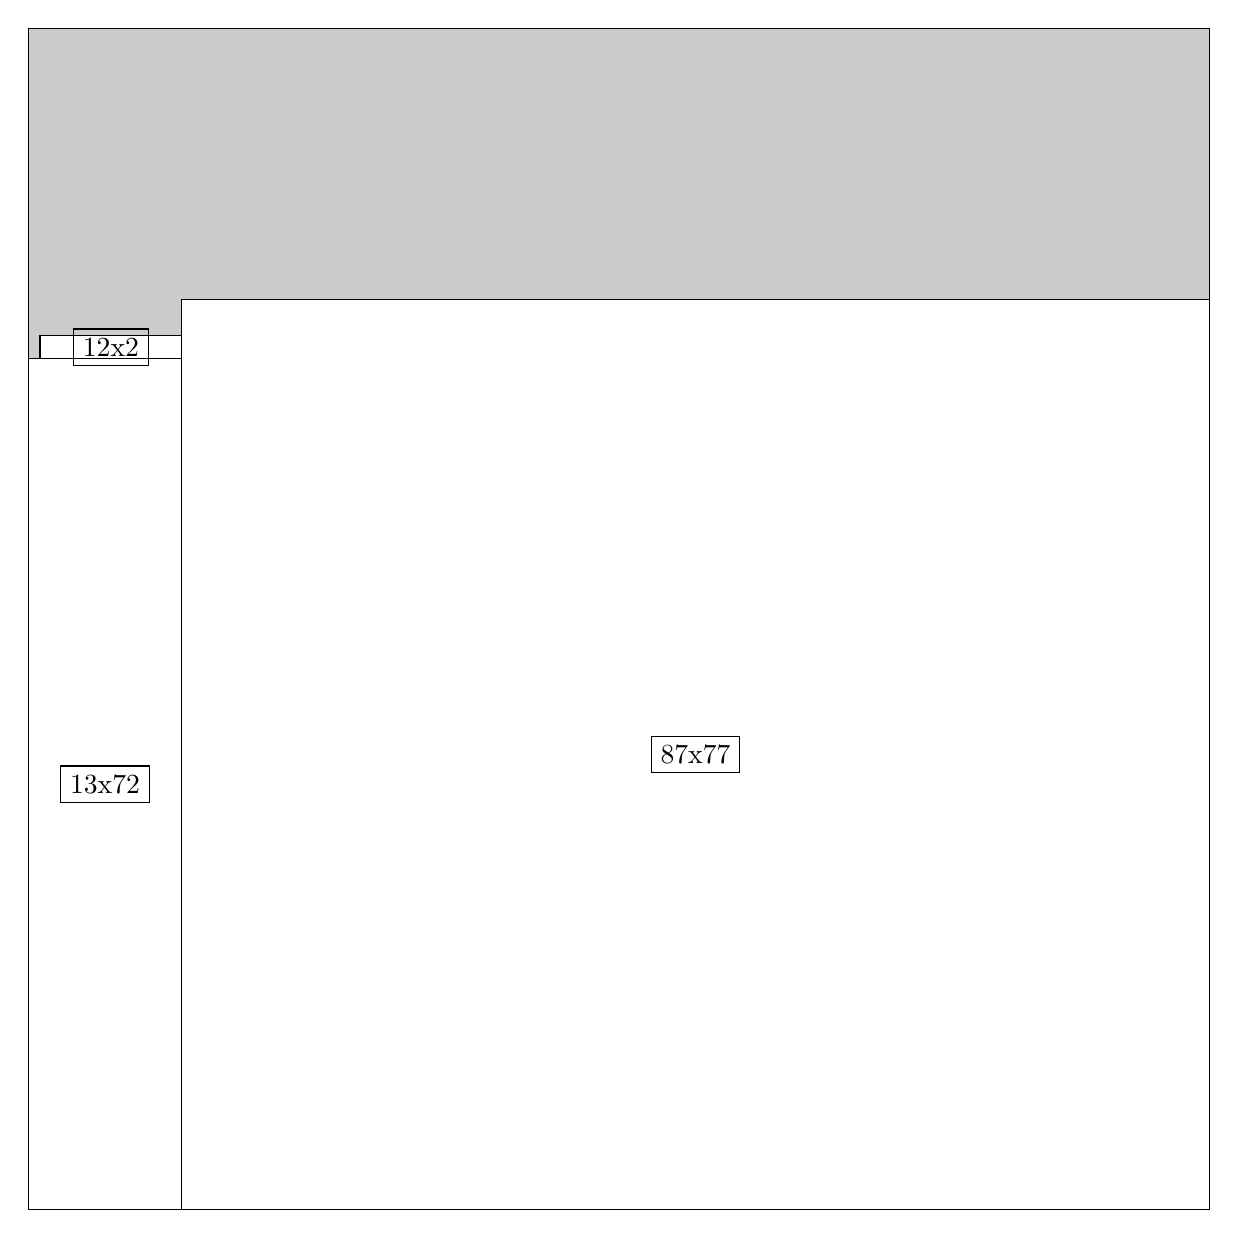
\begin{tikzpicture}[shorten >=1pt,scale=1.0,every node/.style={scale=1.0},->]
\tikzstyle{vertex}=[circle,fill=black!25,minimum size=14pt,inner sep=0pt]
\filldraw[fill=gray!40!white, draw=black] (0,0) rectangle (15.0,15.0);
\foreach \name/\x/\y/\w/\h in {87x77/1.95/0.0/13.049999999999999/11.549999999999999,13x72/0.0/0.0/1.95/10.799999999999999,12x2/0.15/10.799999999999999/1.7999999999999998/0.3}
\filldraw[fill=white!40!white, draw=black] (\x,\y) rectangle node[draw] (\name) {\name} ++(\w,\h);
\end{tikzpicture}


w =87 , h =77 , x =13 , y =0 , v =6699
\par
w =13 , h =72 , x =0 , y =0 , v =936
\par
w =12 , h =2 , x =1 , y =72 , v =24
\par
\newpage


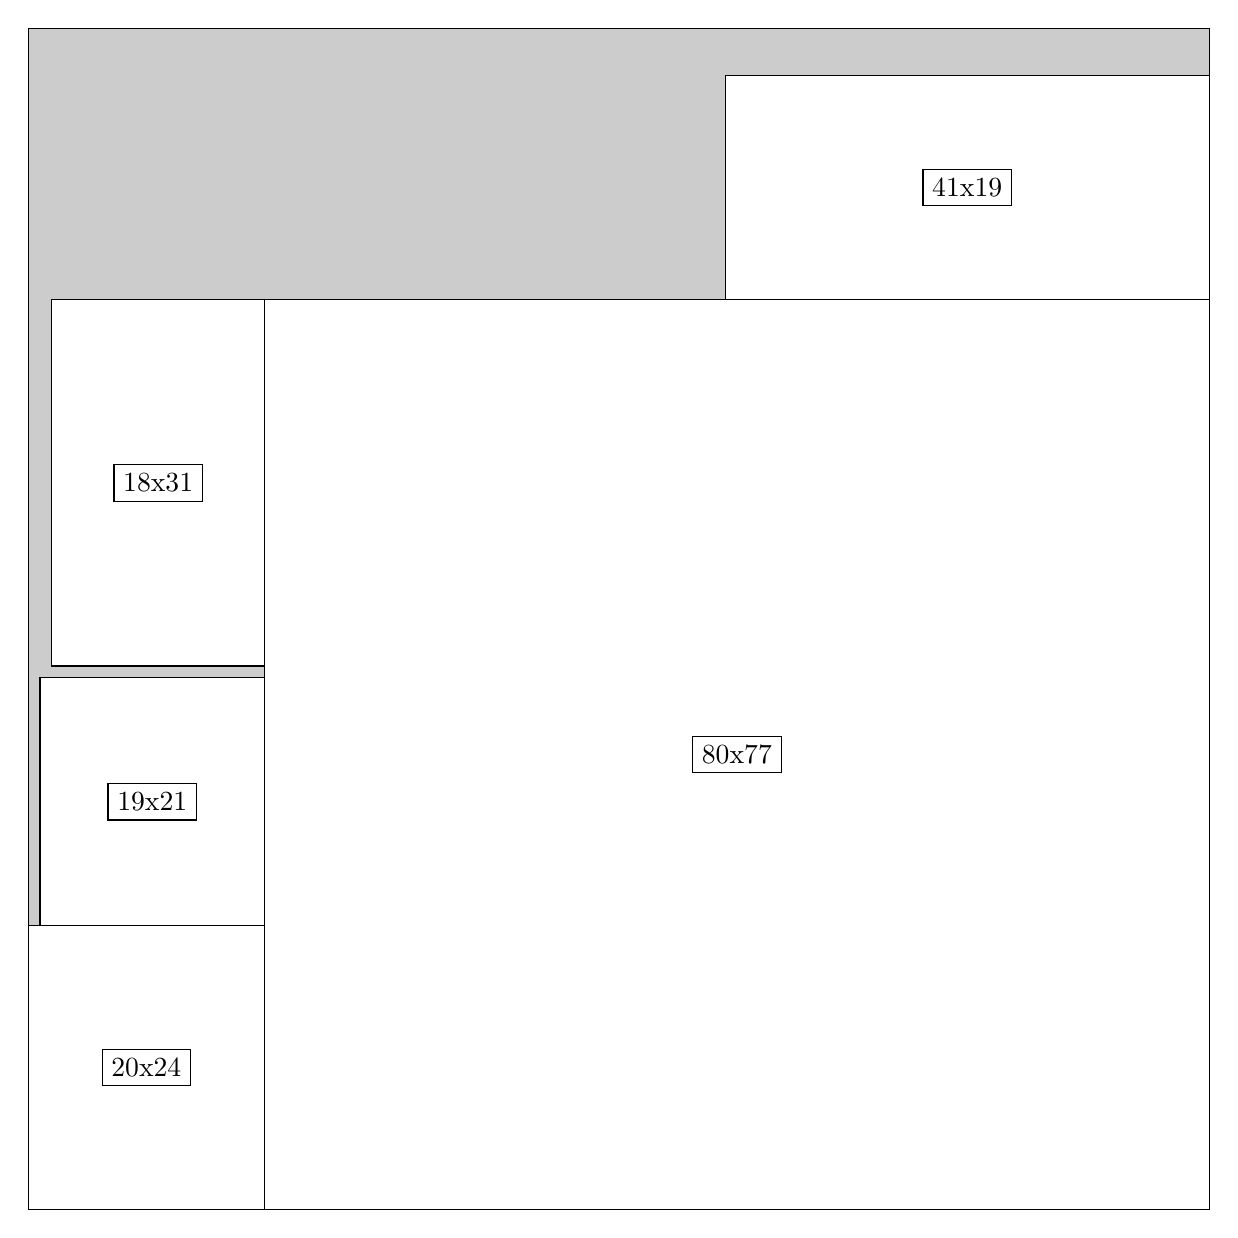
\begin{tikzpicture}[shorten >=1pt,scale=1.0,every node/.style={scale=1.0},->]
\tikzstyle{vertex}=[circle,fill=black!25,minimum size=14pt,inner sep=0pt]
\filldraw[fill=gray!40!white, draw=black] (0,0) rectangle (15.0,15.0);
\foreach \name/\x/\y/\w/\h in {80x77/3.0/0.0/12.0/11.549999999999999,20x24/0.0/0.0/3.0/3.5999999999999996,19x21/0.15/3.5999999999999996/2.85/3.15,18x31/0.3/6.8999999999999995/2.6999999999999997/4.6499999999999995,41x19/8.85/11.549999999999999/6.1499999999999995/2.85}
\filldraw[fill=white!40!white, draw=black] (\x,\y) rectangle node[draw] (\name) {\name} ++(\w,\h);
\end{tikzpicture}


w =80 , h =77 , x =20 , y =0 , v =6160
\par
w =20 , h =24 , x =0 , y =0 , v =480
\par
w =19 , h =21 , x =1 , y =24 , v =399
\par
w =18 , h =31 , x =2 , y =46 , v =558
\par
w =41 , h =19 , x =59 , y =77 , v =779
\par
\newpage


\begin{tikzpicture}[shorten >=1pt,scale=1.0,every node/.style={scale=1.0},->]
\tikzstyle{vertex}=[circle,fill=black!25,minimum size=14pt,inner sep=0pt]
\filldraw[fill=gray!40!white, draw=black] (0,0) rectangle (15.0,15.0);
\foreach \name/\x/\y/\w/\h in {99x81/0.15/0.0/14.85/12.15,96x19/0.6/12.15/14.399999999999999/2.85}
\filldraw[fill=white!40!white, draw=black] (\x,\y) rectangle node[draw] (\name) {\name} ++(\w,\h);
\end{tikzpicture}


w =99 , h =81 , x =1 , y =0 , v =8019
\par
w =96 , h =19 , x =4 , y =81 , v =1824
\par
\newpage


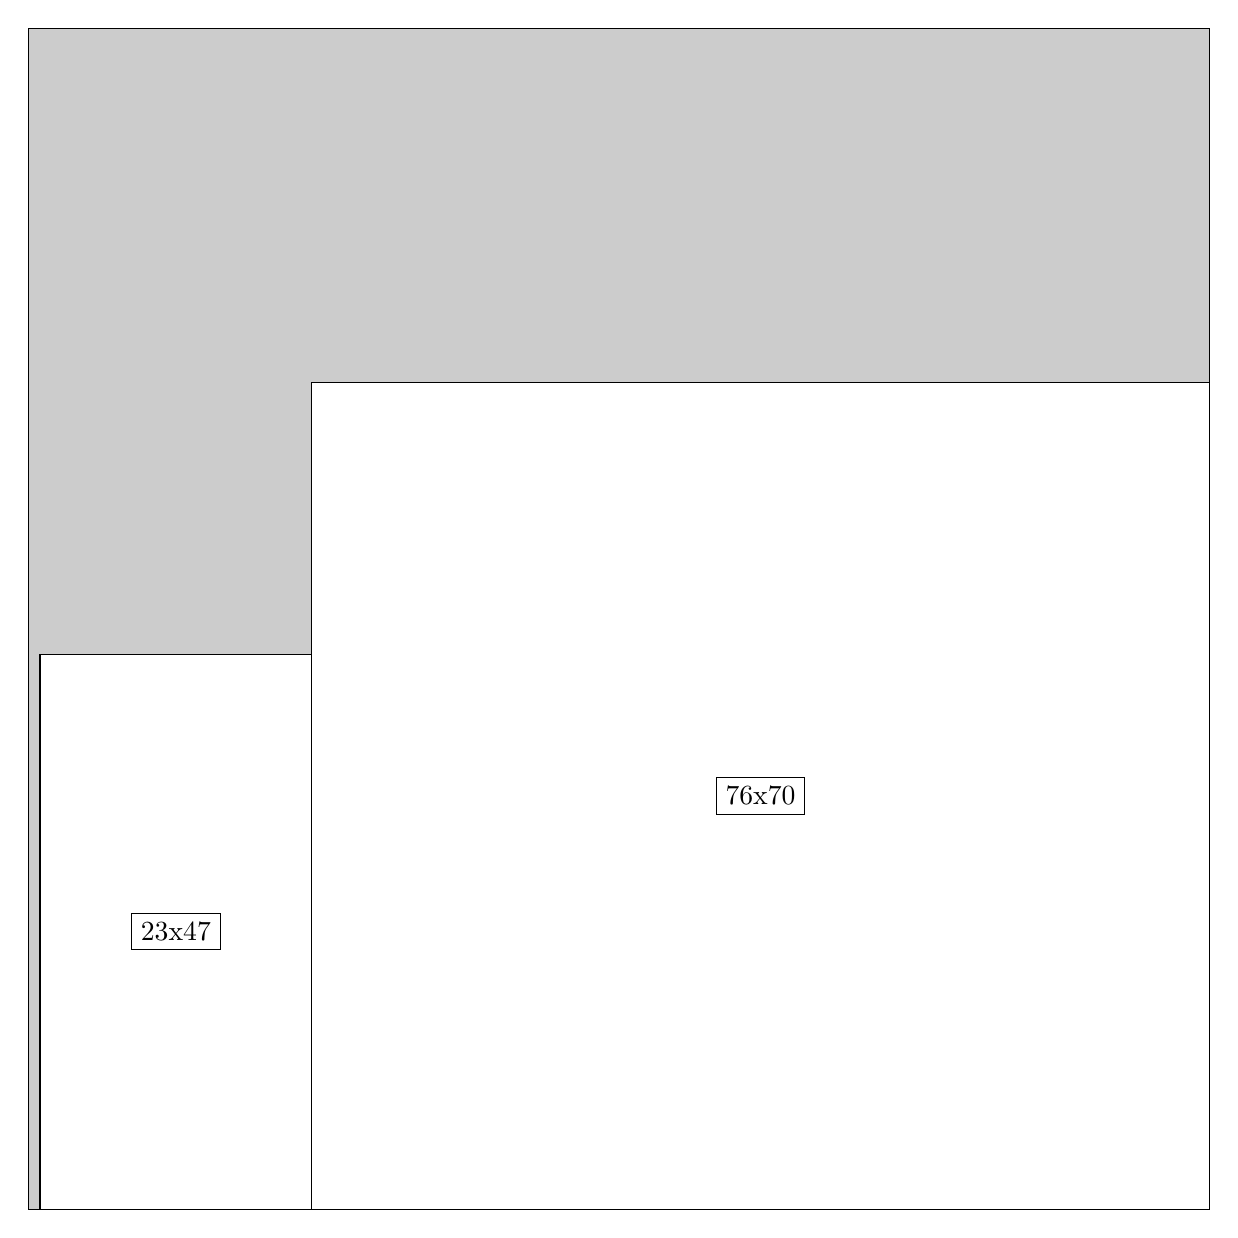
\begin{tikzpicture}[shorten >=1pt,scale=1.0,every node/.style={scale=1.0},->]
\tikzstyle{vertex}=[circle,fill=black!25,minimum size=14pt,inner sep=0pt]
\filldraw[fill=gray!40!white, draw=black] (0,0) rectangle (15.0,15.0);
\foreach \name/\x/\y/\w/\h in {76x70/3.5999999999999996/0.0/11.4/10.5,23x47/0.15/0.0/3.4499999999999997/7.05}
\filldraw[fill=white!40!white, draw=black] (\x,\y) rectangle node[draw] (\name) {\name} ++(\w,\h);
\end{tikzpicture}


w =76 , h =70 , x =24 , y =0 , v =5320
\par
w =23 , h =47 , x =1 , y =0 , v =1081
\par
\newpage


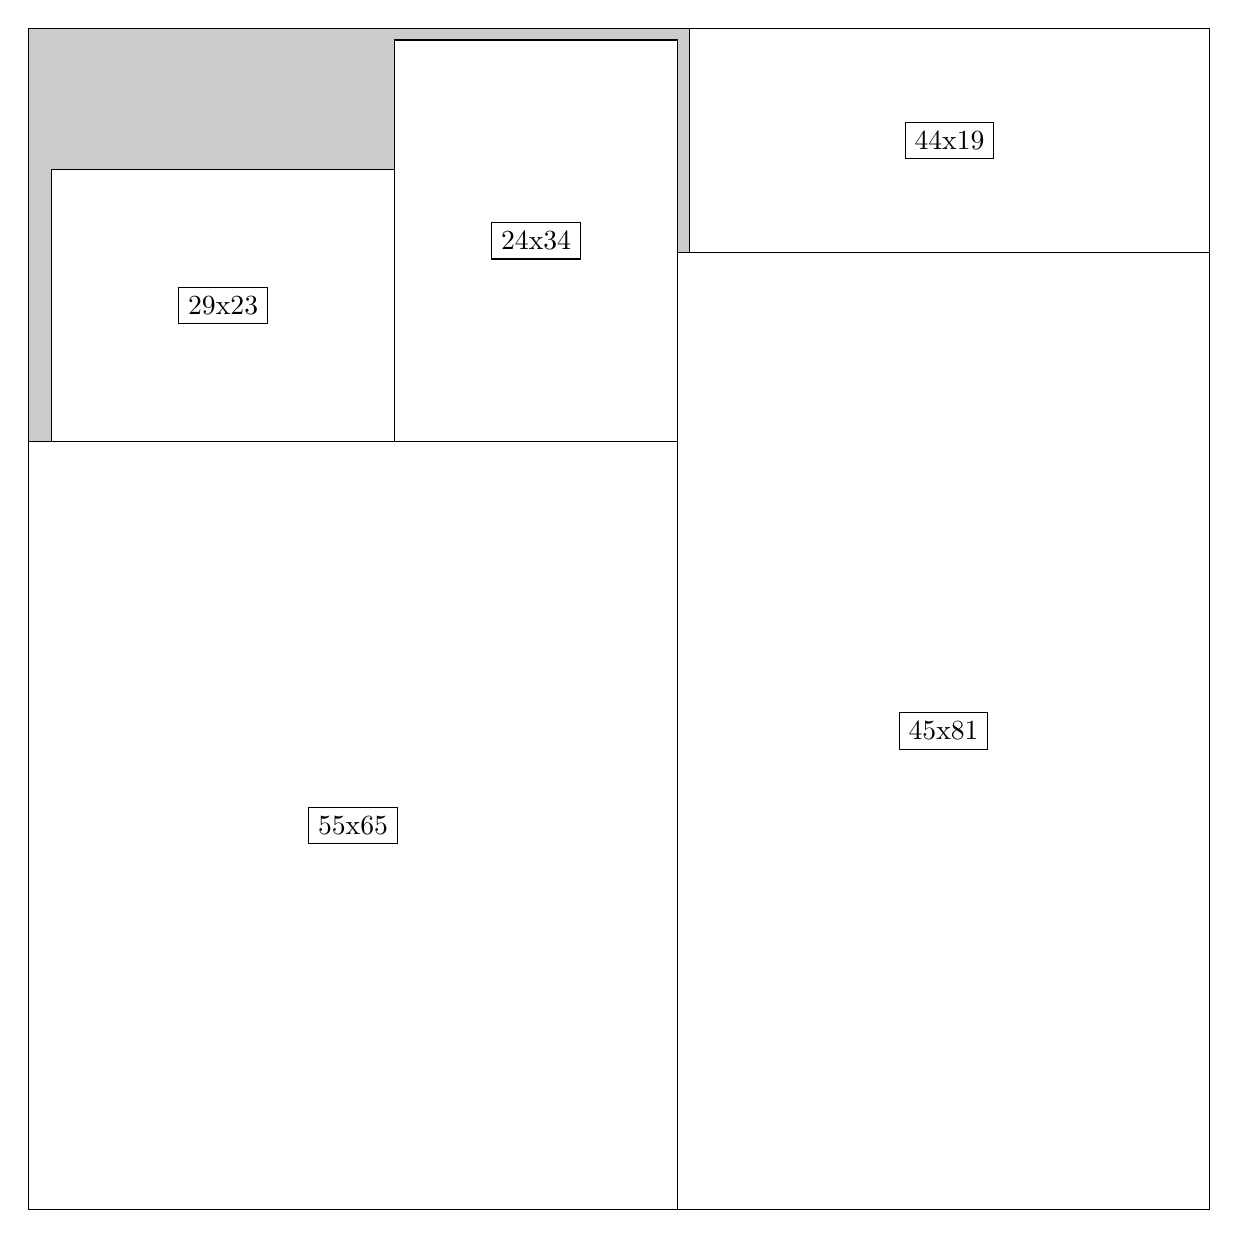
\begin{tikzpicture}[shorten >=1pt,scale=1.0,every node/.style={scale=1.0},->]
\tikzstyle{vertex}=[circle,fill=black!25,minimum size=14pt,inner sep=0pt]
\filldraw[fill=gray!40!white, draw=black] (0,0) rectangle (15.0,15.0);
\foreach \name/\x/\y/\w/\h in {45x81/8.25/0.0/6.75/12.15,44x19/8.4/12.15/6.6/2.85,55x65/0.0/0.0/8.25/9.75,24x34/4.6499999999999995/9.75/3.5999999999999996/5.1,29x23/0.3/9.75/4.35/3.4499999999999997}
\filldraw[fill=white!40!white, draw=black] (\x,\y) rectangle node[draw] (\name) {\name} ++(\w,\h);
\end{tikzpicture}


w =45 , h =81 , x =55 , y =0 , v =3645
\par
w =44 , h =19 , x =56 , y =81 , v =836
\par
w =55 , h =65 , x =0 , y =0 , v =3575
\par
w =24 , h =34 , x =31 , y =65 , v =816
\par
w =29 , h =23 , x =2 , y =65 , v =667
\par
\newpage


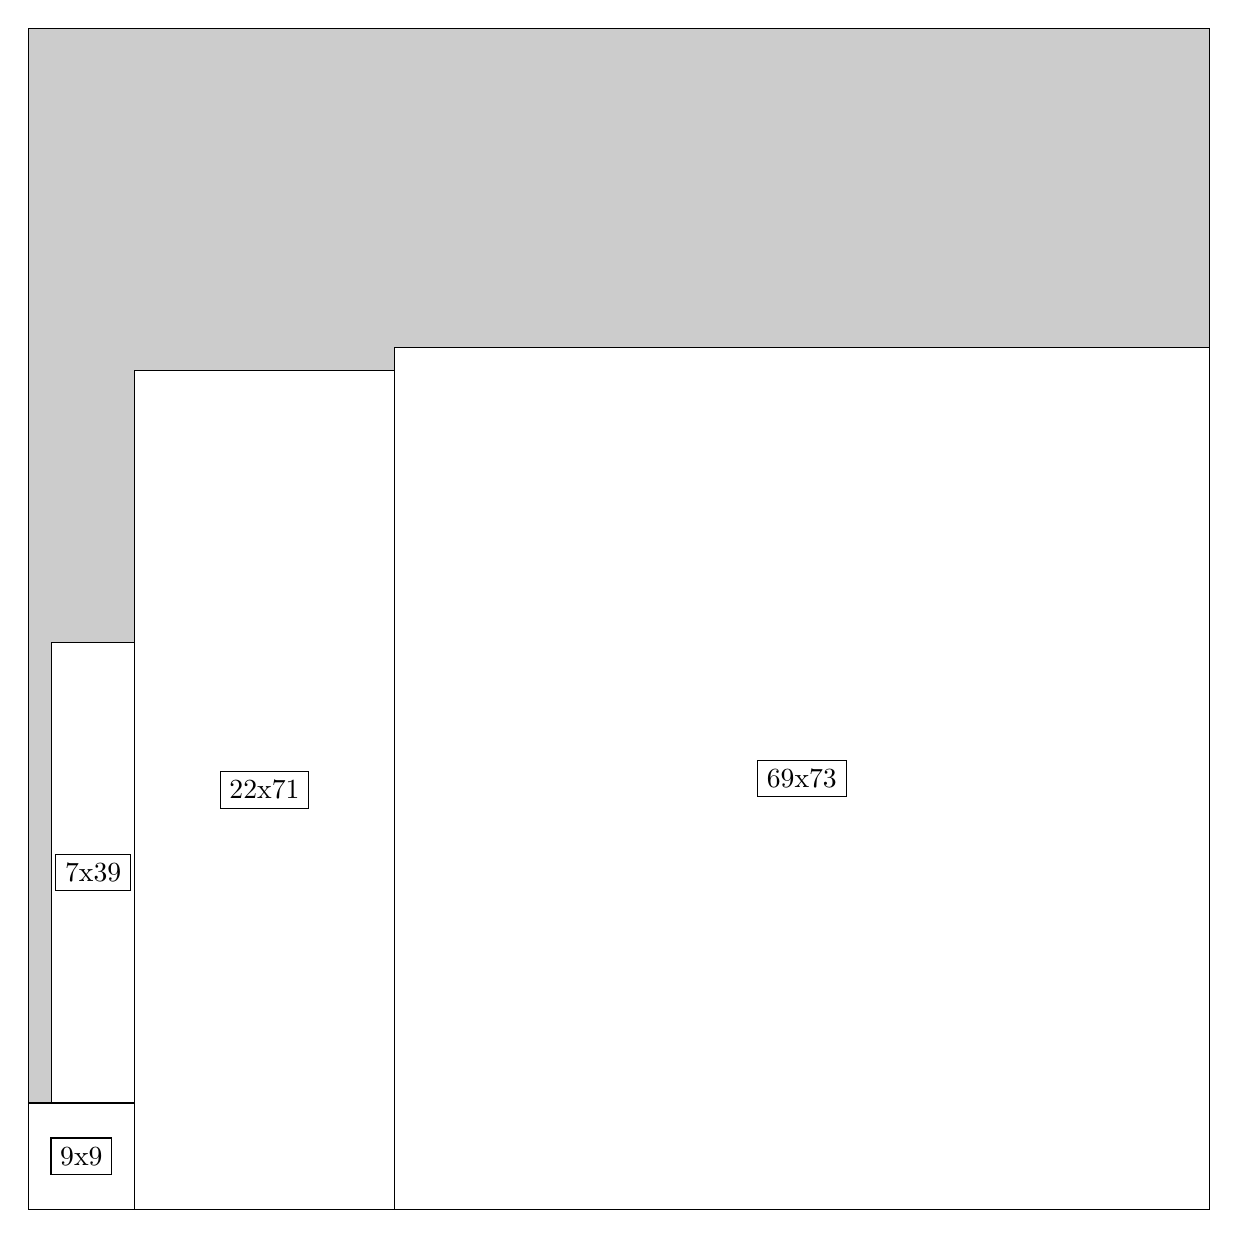
\begin{tikzpicture}[shorten >=1pt,scale=1.0,every node/.style={scale=1.0},->]
\tikzstyle{vertex}=[circle,fill=black!25,minimum size=14pt,inner sep=0pt]
\filldraw[fill=gray!40!white, draw=black] (0,0) rectangle (15.0,15.0);
\foreach \name/\x/\y/\w/\h in {69x73/4.6499999999999995/0.0/10.35/10.95,22x71/1.3499999999999999/0.0/3.3/10.65,9x9/0.0/0.0/1.3499999999999999/1.3499999999999999,7x39/0.3/1.3499999999999999/1.05/5.85}
\filldraw[fill=white!40!white, draw=black] (\x,\y) rectangle node[draw] (\name) {\name} ++(\w,\h);
\end{tikzpicture}


w =69 , h =73 , x =31 , y =0 , v =5037
\par
w =22 , h =71 , x =9 , y =0 , v =1562
\par
w =9 , h =9 , x =0 , y =0 , v =81
\par
w =7 , h =39 , x =2 , y =9 , v =273
\par
\newpage


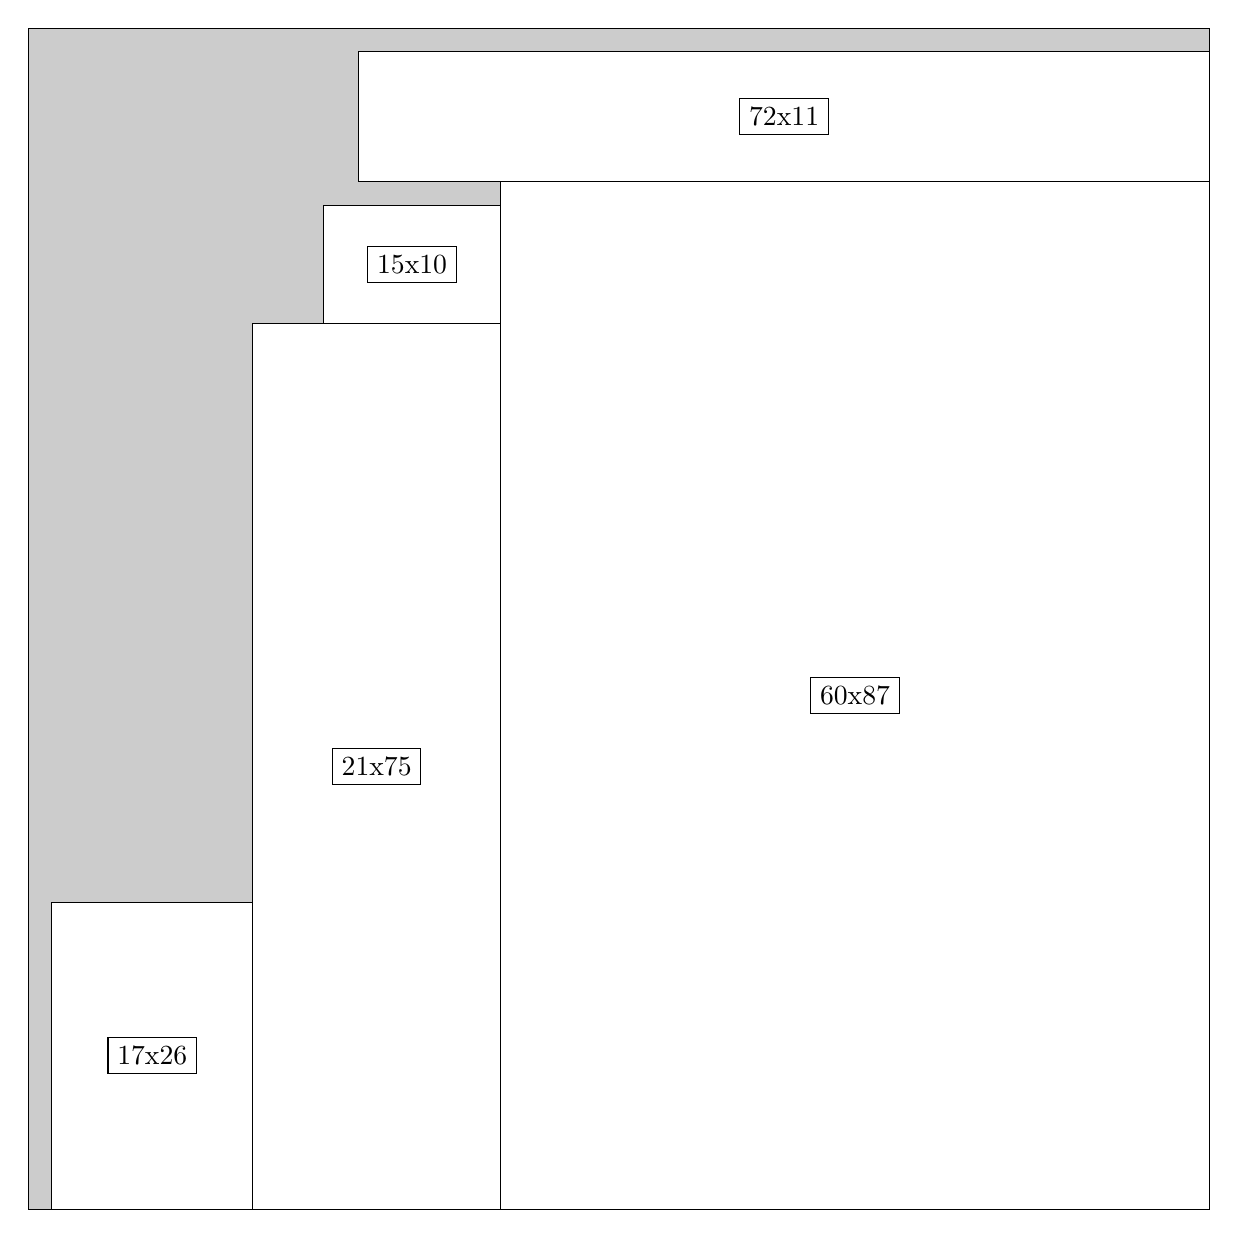
\begin{tikzpicture}[shorten >=1pt,scale=1.0,every node/.style={scale=1.0},->]
\tikzstyle{vertex}=[circle,fill=black!25,minimum size=14pt,inner sep=0pt]
\filldraw[fill=gray!40!white, draw=black] (0,0) rectangle (15.0,15.0);
\foreach \name/\x/\y/\w/\h in {60x87/6.0/0.0/9.0/13.049999999999999,21x75/2.85/0.0/3.15/11.25,15x10/3.75/11.25/2.25/1.5,17x26/0.3/0.0/2.55/3.9,72x11/4.2/13.049999999999999/10.799999999999999/1.65}
\filldraw[fill=white!40!white, draw=black] (\x,\y) rectangle node[draw] (\name) {\name} ++(\w,\h);
\end{tikzpicture}


w =60 , h =87 , x =40 , y =0 , v =5220
\par
w =21 , h =75 , x =19 , y =0 , v =1575
\par
w =15 , h =10 , x =25 , y =75 , v =150
\par
w =17 , h =26 , x =2 , y =0 , v =442
\par
w =72 , h =11 , x =28 , y =87 , v =792
\par
\newpage


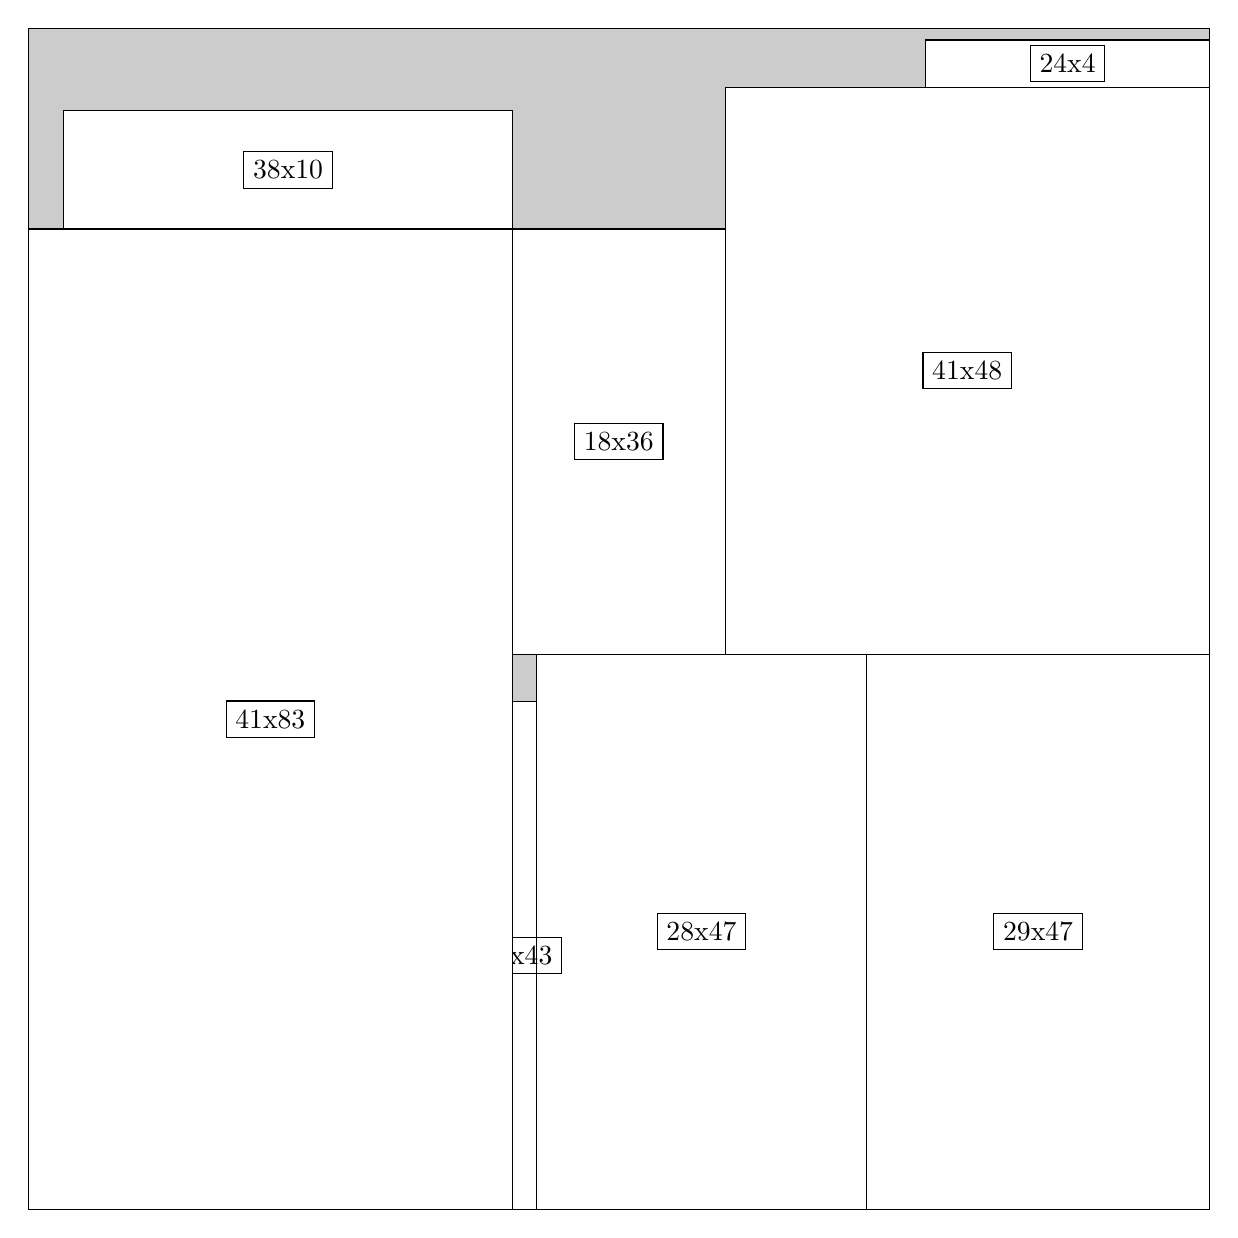
\begin{tikzpicture}[shorten >=1pt,scale=1.0,every node/.style={scale=1.0},->]
\tikzstyle{vertex}=[circle,fill=black!25,minimum size=14pt,inner sep=0pt]
\filldraw[fill=gray!40!white, draw=black] (0,0) rectangle (15.0,15.0);
\foreach \name/\x/\y/\w/\h in {29x47/10.65/0.0/4.35/7.05,28x47/6.45/0.0/4.2/7.05,2x43/6.1499999999999995/0.0/0.3/6.45,41x48/8.85/7.05/6.1499999999999995/7.199999999999999,24x4/11.4/14.25/3.5999999999999996/0.6,18x36/6.1499999999999995/7.05/2.6999999999999997/5.3999999999999995,41x83/0.0/0.0/6.1499999999999995/12.45,38x10/0.44999999999999996/12.45/5.7/1.5}
\filldraw[fill=white!40!white, draw=black] (\x,\y) rectangle node[draw] (\name) {\name} ++(\w,\h);
\end{tikzpicture}


w =29 , h =47 , x =71 , y =0 , v =1363
\par
w =28 , h =47 , x =43 , y =0 , v =1316
\par
w =2 , h =43 , x =41 , y =0 , v =86
\par
w =41 , h =48 , x =59 , y =47 , v =1968
\par
w =24 , h =4 , x =76 , y =95 , v =96
\par
w =18 , h =36 , x =41 , y =47 , v =648
\par
w =41 , h =83 , x =0 , y =0 , v =3403
\par
w =38 , h =10 , x =3 , y =83 , v =380
\par
\newpage


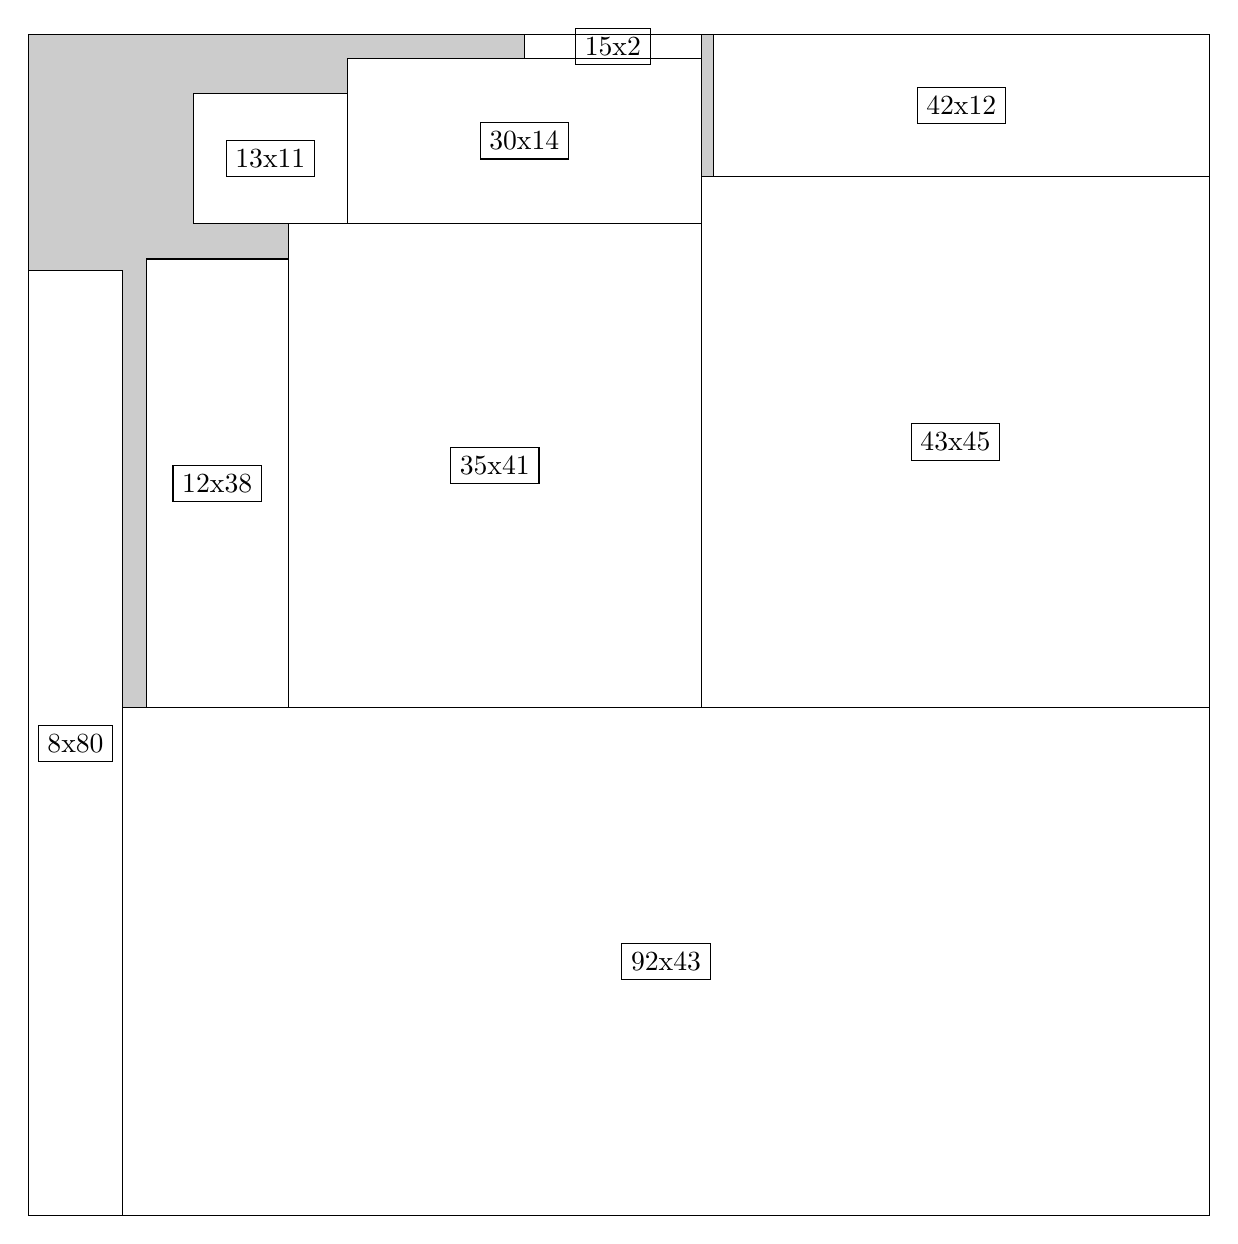
\begin{tikzpicture}[shorten >=1pt,scale=1.0,every node/.style={scale=1.0},->]
\tikzstyle{vertex}=[circle,fill=black!25,minimum size=14pt,inner sep=0pt]
\filldraw[fill=gray!40!white, draw=black] (0,0) rectangle (15.0,15.0);
\foreach \name/\x/\y/\w/\h in {92x43/1.2/0.0/13.799999999999999/6.45,43x45/8.549999999999999/6.45/6.45/6.75,42x12/8.7/13.2/6.3/1.7999999999999998,35x41/3.3/6.45/5.25/6.1499999999999995,12x38/1.5/6.45/1.7999999999999998/5.7,30x14/4.05/12.6/4.5/2.1,15x2/6.3/14.7/2.25/0.3,13x11/2.1/12.6/1.95/1.65,8x80/0.0/0.0/1.2/12.0}
\filldraw[fill=white!40!white, draw=black] (\x,\y) rectangle node[draw] (\name) {\name} ++(\w,\h);
\end{tikzpicture}


w =92 , h =43 , x =8 , y =0 , v =3956
\par
w =43 , h =45 , x =57 , y =43 , v =1935
\par
w =42 , h =12 , x =58 , y =88 , v =504
\par
w =35 , h =41 , x =22 , y =43 , v =1435
\par
w =12 , h =38 , x =10 , y =43 , v =456
\par
w =30 , h =14 , x =27 , y =84 , v =420
\par
w =15 , h =2 , x =42 , y =98 , v =30
\par
w =13 , h =11 , x =14 , y =84 , v =143
\par
w =8 , h =80 , x =0 , y =0 , v =640
\par
\newpage


\end{document}